\documentclass[11pt]{article}

\usepackage[a4paper,margin=1in]{geometry}
\usepackage{microtype}
\usepackage{graphicx}
\usepackage{booktabs}
\usepackage{amsmath}
\usepackage{amssymb}
\usepackage{xcolor}
\usepackage{caption}
\usepackage{subcaption}
\usepackage{enumitem}
\usepackage[hidelinks]{hyperref}
\usepackage{url}
\usepackage{placeins}
\usepackage{titling}
\usepackage{authblk}
\usepackage{epigraph}
\usepackage{fancyhdr}

\setlength{\epigraphwidth}{0.78\textwidth}
\renewcommand{\epigraphflush}{flushleft}
\renewcommand{\epigraphrule}{0pt}

\pagestyle{fancy}
\fancyhf{}
\fancyhead[L]{\small DOWSING}
\fancyhead[R]{\small White-box monitoring in nanoGPT}
\fancyfoot[C]{\thepage}
\renewcommand{\headrulewidth}{0.2pt}

\captionsetup{font=small,labelfont=bf}

\title{\textbf{DOWSING}\\[0.25em]\large Detecting Out-of-Distribution and Weird States in NanoGPT}
\author{Davis Keene}
\affil{\small \texttt{github.com/daviskeene/dowsing}}
\date{May 2026}

\begin{document}

\maketitle
\thispagestyle{fancy}

\begin{abstract}
\noindent
We train a 6-layer, byte-level nanoGPT on Tiny Shakespeare and ask whether its frozen residual-stream activations contain signal that is predictive of token-level surprise and distribution shift, beyond what is recoverable from the output softmax. The headline finding is that the right white-box detector depends on whether the failure family was seen during training: a supervised linear probe wins decisively when its training set covers the test-time shift, an unsupervised Mahalanobis detector on early-layer activations wins when it does not, and the gap between these two regimes is the most informative thing in the experiment. Concretely, on a seen-shift OOD task spanning five synthetic distributions, a layer-5 logistic probe reaches $0.879$ AUROC versus $0.566$ for entropy; under leave-one-shift-out evaluation the probe still beats entropy on $4$ of $5$ held-out families but fails on character-shuffled Shakespeare ($0.590$ AUROC vs.\ $0.603$), where Mahalanobis distance from the ID activation mean recovers $0.696$. A separate within-distribution check (no shift, only token-level surprise) gives the cleanest individual positive result: a layer-4 logistic probe reaches $0.779$ AUROC for held-out Shakespeare high-loss tokens versus $0.656$ for entropy. Diagonal-Laplace Bayesian uncertainty, under fixed prior precision $\tau=1$, is numerically indistinguishable from the deterministic logistic readout at the reported precision; we flag the prior precision (not just the diagonal posterior) as a load-bearing assumption. The verdict is small but specific: hidden states expose token-level failure signals that entropy does not surface, and the choice of monitor must be matched to what the training labels are expected to cover.
\end{abstract}

\epigraph{\itshape A dowsing rod is a folk object: a forked stick that is supposed to twitch when you walk over running water underground. This paper asks the same question, minus the superstition --- can we build a rod that twitches when a language model passes over hidden trouble?}{}

\section{Introduction}

A language model, at the level we study here, has one job: read some tokens and predict the next one. Because the model in this paper is byte-level and trained on a small Shakespeare corpus, the next token is literally the next byte. This compression of the prediction problem to a single character lets us define ``trouble'' very plainly. A token is trouble if the model is about to do badly on it: either because the prefix is ordinary Shakespeare and the model still gets it wrong (high loss), or because the prefix is itself outside the training distribution (OOD).

The standard monitor for this kind of trouble is the output softmax. If the softmax distribution has high entropy, the model looks uncertain; if one token captures most of the mass, it looks confident. The question we ask is whether output confidence is the full story, or whether hidden states contain failure-predictive signal that output entropy does not surface. The hypothesis is that frozen residual-stream activations, read through a small linear probe, expose warning signals that simple softmax-derived confidence metrics do not.

This is a deliberately small experiment. The model is undertrained, the dataset is a small Shakespeare corpus, the OOD sets are partly synthetic, and the probes are linear. What we want is not a strong claim about frontier models. We want a clean enough setup that every step is auditable, and that the negative results are as legible as the positive ones. The intended audience is anyone who, like the author, wants a worked example of white-box monitoring in a system small enough to hold in their head.

\paragraph{Contributions.} We (i)~specify a tiny, end-to-end harness for training a byte-level nanoGPT and recording per-token loss, entropy, max probability, target probability, and post-block residual activations across every transformer layer; (ii)~report a within-distribution high-loss result that survives a stricter audit ($+0.123$ AUROC over entropy at layer~4); (iii)~report a seen-shift OOD result and immediately stress-test it with leave-one-shift-out, where the trained probe degrades and an unsupervised Mahalanobis detector becomes the best deployable monitor for the most adversarial held-out shift; and (iv)~document a negative result for the diagonal-Laplace approximation under fixed prior precision, with the diagonal posterior identified as the load-bearing assumption.

\section{Setup}

\subsection{Model and data}

The language model is a $6$-layer, $6$-head, $192$-dimensional transformer following Karpathy's nanoGPT architecture, with byte-level tokenization and vocabulary size $|\mathcal{V}|=256$, trained on Tiny Shakespeare for $3{,}000$ iterations with batch size $64$ and block size $T=128$ on a single NVIDIA L4 GPU. Final logged validation loss is approximately $1.444$ nats per byte. Byte-level tokenization is convenient here for one structural reason: every distribution shift we cook up still lies inside the input alphabet, so the model is never asked to handle out-of-vocabulary bytes; the only thing that changes is the joint distribution over byte sequences.

\subsection{Per-token observables}

For each evaluation token at position $t$ we record the cross-entropy loss
\begin{equation}
  \ell_t \;=\; -\log p_\theta\!\left(y_t \mid x_{<t}\right),
\end{equation}
the predictive entropy
\begin{equation}
  H_t \;=\; -\sum_{v \in \mathcal{V}} p_\theta(v \mid x_{<t}) \log p_\theta(v \mid x_{<t}),
\end{equation}
the max probability $\max_v p_\theta(v\mid x_{<t})$, the target probability $p_\theta(y_t\mid x_{<t})$, the model's top prediction, and the post-block residual-stream activation $\mathbf{h}_t^{(\ell)} \in \mathbb{R}^{192}$ at every transformer block $\ell \in \{0,1,\dots,5\}$. Note that $\ell_t = -\log p_\theta(y_t\mid x_{<t})$, so target probability and loss are oracle diagnostics for high-loss --- they require knowledge of the true next byte and cannot be used as deployment-time monitors. We retain them in the tables as upper-bound references.

\subsection{Tasks}

We evaluate every detector on two binary classification tasks defined over individual tokens.

\paragraph{High-loss.} A token is labeled positive if $\ell_t$ exceeds the $80$th percentile of held-out in-distribution losses,
\begin{equation}
  y^{\mathrm{HL}}_t \;=\; \mathbf{1}\!\left[\ell_t > q_{0.8}(\ell\,\vert\,\mathrm{ID\ train})\right].
\end{equation}
The threshold is fit on ID training rows only, so the labeling rule does not see the test split.

\paragraph{Out-of-distribution.} A token is labeled positive if its source sequence was drawn from one of five shift families: \texttt{python}, \texttt{modern\_prose}, \texttt{repetition}, \texttt{word\_shuffle}, and \texttt{char\_shuffle}. The first three are template-generated and tiled to fill the eval split; the last two are derived from held-out Shakespeare bytes by shuffling at the character or word level. The shuffled sets are the load-bearing OOD families because they cannot reuse content from the training prefix; we flag the tiled families as engineering stress tests and not natural distribution estimates.

\subsection{Splits and leakage control}\label{sec:splits}

All splits are at the level of fixed-length windows, not individual tokens. Each window is assigned to train, validation, or test as an indivisible unit, so a probe cannot succeed by memorizing its own near-neighbor activations within a window. Neighboring windows from the same source byte stream, produced by sliding the window with a fixed stride, are not separately de-duplicated and can land in different splits; we flag this as a residual leakage channel that future work should close. Every probe is trained on activations from a frozen language model; the model itself is never updated.

\section{Methods}

We compare four families of scores: output baselines, oracle diagnostics, supervised linear probes, and an unsupervised one-class detector. The notation $\mathbf{h}^{(\ell)} \in \mathbb{R}^{d}$ refers to the post-block residual activation at layer $\ell$, with $d=192$.

\subsection{Output baselines and oracle diagnostics}

We separate two kinds of softmax-derived score. \emph{Output baselines} are deployable monitors that depend only on the model's output distribution: predictive entropy $H_t$ and $1-\max_v p_\theta(v\mid x_{<t})$. \emph{Oracle diagnostics} also derive from the output distribution but require the true next byte: the per-token loss $\ell_t$ and the negative target probability $-p_\theta(y_t\mid x_{<t})$. We retain the oracle diagnostics in the tables because they upper-bound the available signal in the softmax, but they are not detectors that could run at generation time. Both groups are ranked scores, not probability outputs, so Brier, NLL, and ECE are intentionally blank for them.

\subsection{Linear probes}

\paragraph{Logistic regression.} A single linear-affine readout per layer, trained with class-weighted cross-entropy. Letting $z_i = \mathbf{w}^\top \mathbf{h}_i^{(\ell)} + b$,
\begin{equation}
  \min_{\mathbf{w},b}\; \sum_{i=1}^{N} w_{y_i}\,\big[\!-y_i \log \sigma(z_i)\,-\,(1-y_i)\log(1-\sigma(z_i))\big] \;+\; \tfrac{1}{2C}\|\mathbf{w}\|_2^{2},
\end{equation}
where $\sigma$ is the logistic function, the per-class weights $w_y$ correct for the $20\%/80\%$ positive/negative imbalance on the high-loss task, and $C$ is a fixed inverse-regularization strength. Because the probe is class-weighted, its sigmoid outputs should be read as scoring outputs rather than calibrated forecasts; AUROC and AUPRC are the primary metrics, calibration is secondary.

\paragraph{Ridge classifier.} A least-squares regression onto $\pm 1$ targets, with $\ell_2$ regularization:
\begin{equation}
  \min_{\mathbf{w},b}\; \sum_{i=1}^{N} \big(\tilde{y}_i - \mathbf{w}^\top \mathbf{h}_i^{(\ell)} - b\big)^{2} + \alpha \|\mathbf{w}\|_{2}^{2},\qquad \tilde{y}_i \in \{-1,+1\}.
\end{equation}
The decision score is the regression output. Useful as a sanity check that the logistic probe's behaviour is not an artefact of the link function.

\paragraph{Activation norm.} Ranked score given by $\|\mathbf{h}^{(\ell)}\|_2$. A standardized variant uses a per-feature z-score against ID statistics. Both are essentially zero-parameter detectors and serve as the lower bound for what the geometry alone provides.

\subsection{Mahalanobis distance from the ID mean}

Following Lee et al.~(2018), we estimate per-layer the in-distribution mean $\boldsymbol{\mu}^{(\ell)}$ and a shrunk covariance $\boldsymbol{\Sigma}^{(\ell)}$ from ID training activations only. The score is
\begin{equation}
  M^{(\ell)}_t \;=\; \big(\mathbf{h}_t^{(\ell)} - \boldsymbol{\mu}^{(\ell)}\big)^{\!\top} \big(\boldsymbol{\Sigma}^{(\ell)}\big)^{\!-1} \big(\mathbf{h}_t^{(\ell)} - \boldsymbol{\mu}^{(\ell)}\big).
\end{equation}
This detector sees \emph{no} OOD examples during fitting; it learns only what the ID activation cloud looks like. It is the natural foil to the supervised probe under leave-one-shift-out, because its training distribution is fixed across all held-out shift settings.

\subsection{Diagonal-Laplace logistic regression}

Following the Laplace-approximation approach of MacKay (1992), we fit a logistic regression as above, then approximate the posterior over weights by a Gaussian centered at the MAP solution $\mathbf{w}^\star$. We restrict the precision to its diagonal,
\begin{equation}
  q(\mathbf{w}) \;=\; \mathcal{N}\!\big(\mathbf{w};\,\mathbf{w}^\star,\, \mathbf{H}_{\mathrm{diag}}^{-1}\big),
\end{equation}
where $\mathbf{H}_{\mathrm{diag}}$ is the diagonal of the negative log-posterior Hessian under fixed prior precision $\tau$. Two predictive scores are derived:
\begin{itemize}[topsep=2pt,itemsep=0pt]
  \item \textbf{Predictive mean.} An MC estimate of $\mathbb{E}_{\mathbf{w}\sim q}\!\left[\sigma(\mathbf{w}^\top \mathbf{h})\right]$, intended to integrate over weight uncertainty.
  \item \textbf{Mutual information (BALD).} The classic decomposition $H[\bar{p}] - \mathbb{E}_{\mathbf{w}\sim q}\!\big[H[\sigma(\mathbf{w}^\top\mathbf{h})]\big]$, which isolates epistemic uncertainty.
\end{itemize}
We name the assumption explicitly: a diagonal Gaussian over weights is a severe approximation when residual-stream features are correlated, which they are. The negative result we report below is conditional on this approximation.

\subsection{Hyperparameters and protocol}\label{sec:hyperparameters}

For reproducibility we list the concrete values used by each detector. All probes operate on standardized features: per-feature mean and standard deviation are estimated from the probe's own training rows and applied to all splits. Logistic regression uses scikit-learn's implementation with $C=1.0$, the L-BFGS solver, a $1{,}000$-iteration cap, and balanced class weights. Ridge classification uses the same library with default $\alpha=1.0$ and the same balanced weighting. The Mahalanobis detector is fit on standardized in-distribution training activations: the empirical covariance is shrunk by adding $\rho I$ with $\rho=10^{-3}$, and the inverse is computed via the Moore--Penrose pseudoinverse for numerical stability. The diagonal-Laplace probe is initialized at the logistic MAP solution with a fixed prior precision $\tau=1.0$, and its predictive scores are estimated from $S=64$ Monte Carlo samples of the weight posterior. Sequence-level splits are $60/20/20$ train/validation/test, with each fixed-length window assigned as an indivisible unit. This prevents token-level leakage within a window; neighboring windows from the same source byte stream are not separately de-duplicated and may land in different splits.

\paragraph{Layer selection.} Layer-best tables (Tables~\ref{tab:idonly}, \ref{tab:fairood}, \ref{tab:loso}, \ref{tab:loso-best}) report the layer with the highest test-split AUROC for each detector. The validation split is held out from probe training but is not used for layer selection in the current pipeline. These tables are therefore descriptive and may be mildly optimistic relative to a protocol that selects layers on validation and reports once on test. For the LOSO setting, the same selection rule is applied within each held-out shift evaluation, so the optimism is uniform across detectors and does not advantage one over another.

\subsection{Evaluation metrics}

We report AUROC and AUPRC as primary metrics. For probability outputs we additionally report Brier score, NLL, and expected calibration error (ECE). Because the supervised logistic probes are trained with class weighting, their sigmoid outputs are not calibrated probabilities; we include Brier and ECE for them only as rough diagnostics, not as the metric of record. Calibration metrics are deliberately blank for ranked scores --- entropy, loss, distances, norms --- where they are not defined.

\section{Results}

\subsection{Within-distribution token surprise (H1)}

The cleanest result is the ID-only high-loss check. The probe is trained on activations from held-out Shakespeare windows alone, with the high-loss threshold fit from ID train rows. Table~\ref{tab:idonly} reports the layer-best detector for each method; Figure~\ref{fig:high_loss_layers} shows the layer sweep.

\begin{table}[h]
  \centering
  \small
  \begin{tabular}{lcccccc}
    \toprule
    Method & Layer & AUROC & AUPRC & Brier & ECE & $n_{\mathrm{test}}$ \\
    \midrule
    Deterministic logistic       & 4 & \textbf{0.779} & 0.517 & 0.184 & 0.221 & 9{,}960 \\
    Laplace predictive mean      & 4 & 0.779 & 0.517 & 0.184 & 0.221 & 9{,}960 \\
    Ridge classifier             & 4 & 0.780 & 0.509 & ---   & ---   & 9{,}960 \\
    Entropy (output baseline)    & --- & 0.656 & 0.321 & ---   & ---   & 9{,}960 \\
    $1-\max p$ (output baseline) & --- & 0.638 & 0.298 & ---   & ---   & 9{,}960 \\
    Mahalanobis                  & 0 & 0.594 & 0.346 & ---   & ---   & 9{,}960 \\
    Standardized activation norm & 0 & 0.506 & 0.234 & ---   & ---   & 9{,}960 \\
    \bottomrule
  \end{tabular}
  \caption{ID-only high-loss detection. The probe is trained and tested only on held-out Shakespeare windows; the loss threshold is fit from ID train rows. The layer-4 logistic probe beats entropy by $+0.123$ AUROC.}
  \label{tab:idonly}
\end{table}

\begin{figure}[h]
  \centering
  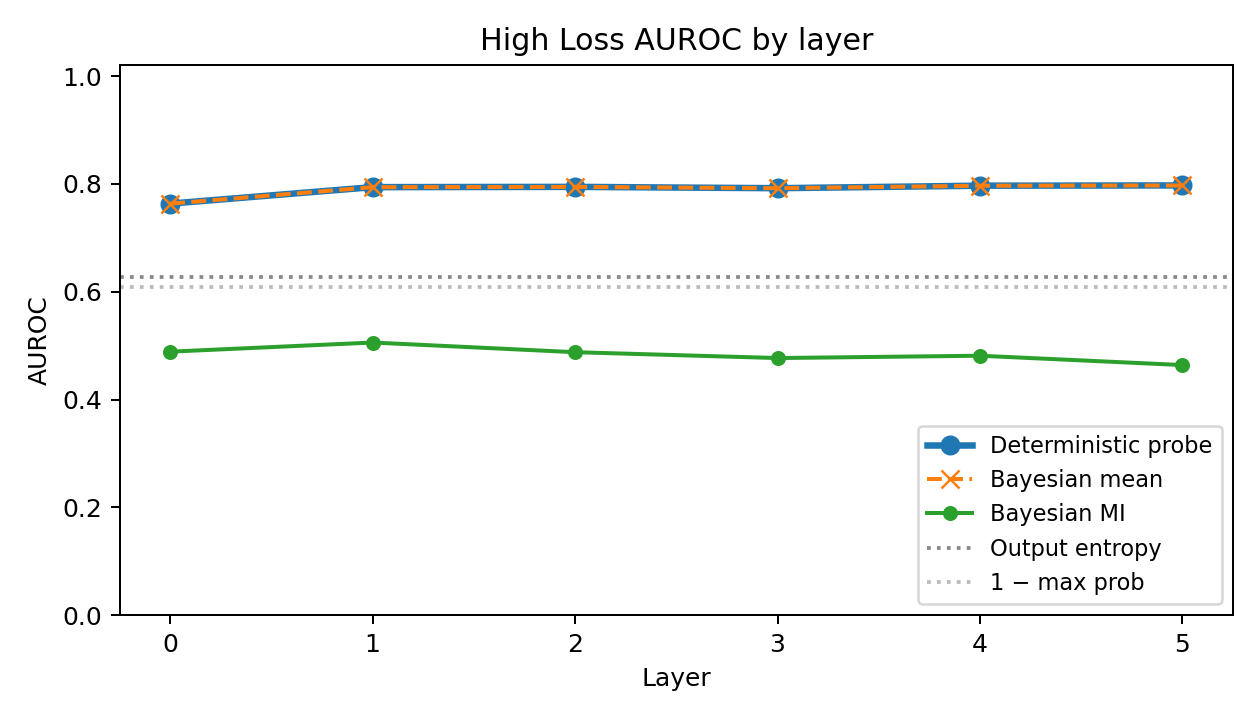
\includegraphics[width=0.85\linewidth]{../artifacts/plots/high_loss_auroc_by_layer.png}
  \caption{High-loss AUROC by layer for each detector. The supervised probe is the dominant signal; output baselines (gray) are flat across layers because they do not depend on activation depth.}
  \label{fig:high_loss_layers}
\end{figure}

This is the least OOD-confounded positive result. The labeling rule never sees the test split, and the input distribution does not change between train and test. Because splits are window-level rather than source-region-level (see~\S\ref{sec:scope}), the result should be read as evidence about held-out windows rather than fully de-duplicated held-out corpus text. Within those bounds, frozen activations carry $0.123$ AUROC of additional ranking signal beyond the output softmax.

\subsection{Seen-shift OOD detection (H2)}

When the probe is trained on examples from \emph{all five} OOD families and tested on more examples from those same families, the layer-5 logistic probe reaches $0.879$ AUROC against entropy at $0.566$ (Table~\ref{tab:fairood}, Figure~\ref{fig:ood_layers}).

\begin{table}[h]
  \centering
  \small
  \begin{tabular}{lcccccl}
    \toprule
    Method & Layer & AUROC & AUPRC & Brier & ECE & note \\
    \midrule
    Deterministic logistic        & 5 & \textbf{0.879} & 0.971 & 0.137 & 0.176 & best layer \\
    Laplace predictive mean       & 5 & 0.879 & 0.971 & 0.137 & 0.176 & best layer \\
    Ridge classifier              & 5 & 0.878 & 0.971 & --- & --- & best layer \\
    Loss (oracle)                 & --- & 0.681 & 0.917 & --- & --- & oracle baseline \\
    $-p(y_t\mid x_{<t})$ (oracle) & --- & 0.681 & 0.917 & --- & --- & oracle baseline \\
    Mahalanobis                   & 1 & 0.629 & 0.894 & --- & --- & best layer \\
    Entropy                       & --- & 0.566 & 0.858 & --- & --- & output baseline \\
    $1-\max p$                    & --- & 0.556 & 0.848 & --- & --- & output baseline \\
    Activation norm               & 0 & 0.486 & 0.843 & --- & --- & best layer \\
    Laplace MI                    & 1 & 0.455 & 0.819 & --- & --- & best layer \\
    \bottomrule
  \end{tabular}
  \caption{Seen-shift OOD detection. The probe has seen examples of every shift family during training. The result is informative as a seen-shift monitor; it is not evidence of generalization to unseen shifts.}
  \label{tab:fairood}
\end{table}

\begin{figure}[h]
  \centering
  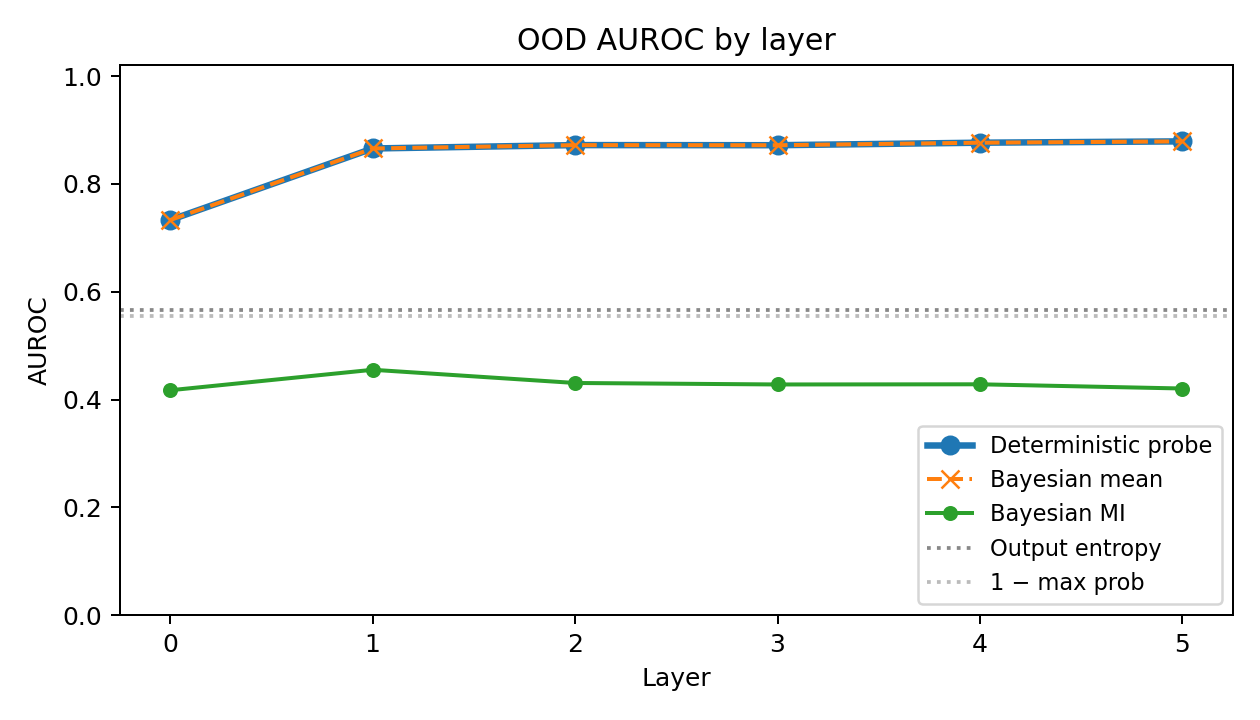
\includegraphics[width=0.85\linewidth]{../artifacts/plots/ood_auroc_by_layer.png}
  \caption{Seen-shift OOD AUROC by layer. Trained probes (blue, orange) dominate output baselines (gray) at every layer. The Bayesian-MI variant (green) sits below $0.5$; this approximation does not produce a useful uncertainty signal in this setup.}
  \label{fig:ood_layers}
\end{figure}

\paragraph{Per-shift breakdown.}
Within the seen-shift task, the layer-5 probe beats entropy on every shift family (Figure~\ref{fig:typebreakdown}; full numbers in Appendix~\ref{app:typebreakdown}). The largest gain is on \texttt{repetition} ($+0.457$ AUROC), the smallest on \texttt{char\_shuffle} ($+0.171$). All five gains are conditional on having seen each shift family during probe training; the leave-one-shift-out section qualifies this immediately.

\begin{figure}[h]
  \centering
  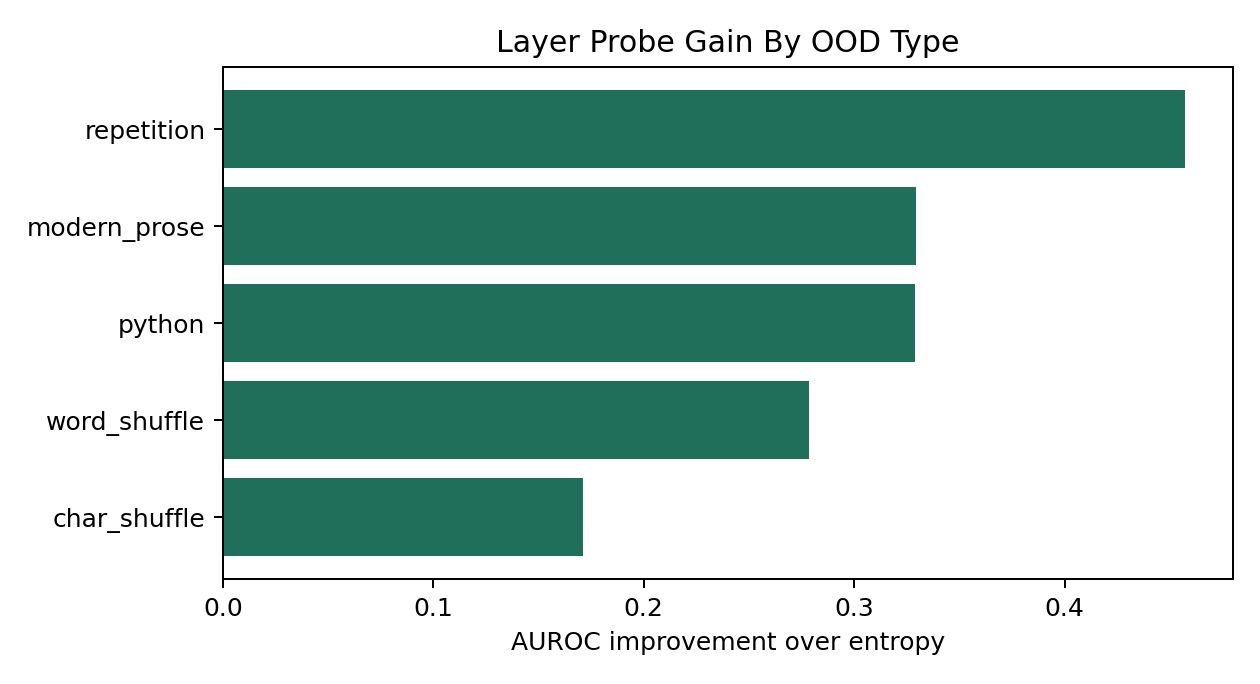
\includegraphics[width=0.85\linewidth]{../artifacts/plots/ood_probe_delta_by_type.png}
  \caption{Probe AUROC minus entropy AUROC, by OOD family, for the layer-5 seen-shift probe (the best aggregate OOD layer). Largest gains are on the easiest families (\texttt{python}, \texttt{repetition}); smallest gain is on \texttt{char\_shuffle}, which is precisely the family that fails to generalize under leave-one-shift-out.}
  \label{fig:typebreakdown}
\end{figure}

\subsection{Held-out-shift OOD generalization (H2, LOSO)}

Seen-shift detection is a weak test: a probe can succeed by learning ``Python looks weird'' rather than ``the model is outside its comfort zone.'' To separate the two, we re-run the probe pipeline holding out one shift family at a time --- the probe trains on ID plus the other four families and is tested on ID plus the held-out fifth. Table~\ref{tab:loso} reports the trained logistic probe under this stricter protocol; Table~\ref{tab:loso-best} reports the best deployable detector per held-out shift, where ``deployable'' excludes oracle baselines.

\begin{table}[!ht]
  \centering
  \footnotesize
  \begin{tabular}{lccccc}
    \toprule
    Held-out shift & Probe layer & Probe AUROC & Entropy AUROC & Loss AUROC \emph{(oracle)} & $\Delta$ vs.\ entropy \\
    \midrule
    \texttt{modern\_prose} & 2 & 0.822 & 0.571 & 0.585 & $+0.251$ \\
    \texttt{repetition}    & 5 & 0.690 & 0.505 & 0.497 & $+0.185$ \\
    \texttt{word\_shuffle} & 4 & 0.729 & 0.554 & 0.629 & $+0.175$ \\
    \texttt{python}        & 5 & 0.747 & 0.591 & 0.783 & $+0.156$ \\
    \texttt{char\_shuffle} & 5 & 0.590 & 0.603 & 0.898 & $-0.013$ \\
    \bottomrule
  \end{tabular}
  \caption{Leave-one-OOD-type-out: the probe is trained on four shift families and tested on the held-out fifth plus held-out ID. The trained probe beats entropy on $4$ of $5$ held-out shifts; on \texttt{char\_shuffle}, which had been presented as the most controlled sanity check, it underperforms entropy.}
  \label{tab:loso}
\end{table}

\begin{table}[h]
  \centering
  \small
  \begin{tabular}{llcc}
    \toprule
    Held-out shift & Best deployable detector & Layer & AUROC \\
    \midrule
    \texttt{python}        & Mahalanobis     & 1 & \textbf{0.858} \\
    \texttt{modern\_prose} & Ridge classifier & 2 & \textbf{0.829} \\
    \texttt{word\_shuffle} & Ridge classifier & 4 & 0.739 \\
    \texttt{char\_shuffle} & Mahalanobis     & 0 & \textbf{0.696} \\
    \texttt{repetition}    & Logistic probe  & 5 & 0.690 \\
    \bottomrule
  \end{tabular}
  \caption{Best observed deployable detector for each held-out shift, selected in hindsight after seeing the held-out results. Oracle scores (\texttt{loss}, $-p(y_t)$) are excluded because they require the true next byte. On \texttt{char\_shuffle} and \texttt{python}, the unsupervised Mahalanobis detector --- which has seen no OOD examples at all --- generalizes better than the supervised probe.}
  \label{tab:loso-best}
\end{table}

\begin{figure}[h]
  \centering
  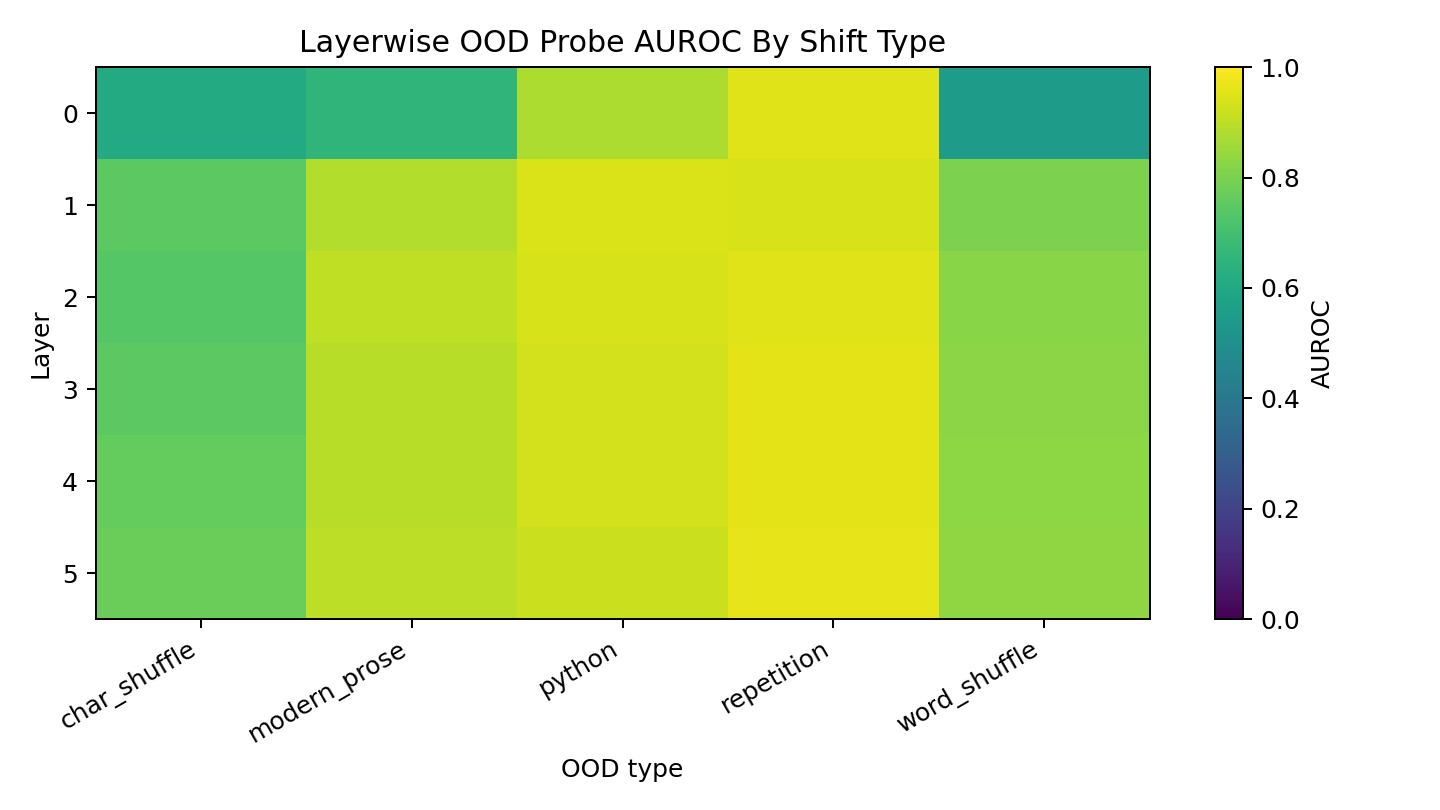
\includegraphics[width=0.92\linewidth]{../artifacts/plots/ood_layer_type_heatmap.png}
  \caption{Layer-by-shift AUROC heatmap. \texttt{python} and \texttt{modern\_prose} become linearly accessible at earlier or middle layers; \texttt{repetition}, \texttt{word\_shuffle}, and \texttt{char\_shuffle} are strongest at the final layer. There is no single ``monitoring layer'' that is best for every shift.}
  \label{fig:layerheat}
\end{figure}

\paragraph{The \texttt{char\_shuffle} row.} \texttt{char\_shuffle} is the most controlled of the five shifts: the bytes come from held-out Shakespeare and are merely permuted within a sequence, so there is no novel content to learn at the byte level. Under the seen-shift task, the probe achieves $+0.171$ AUROC over entropy on this family. Under leave-one-shift-out, that gain inverts to $-0.013$. The honest reading is that the seen-shift gain is consistent with the probe learning a shift-family-specific direction --- one that fits \texttt{char\_shuffle} when its examples are in training --- rather than a general OOD direction. Mahalanobis distance at layer~$0$ recovers $0.696$ AUROC on the same held-out test, so the activation geometry does carry a usable signal for this shift; the supervised probe is simply pointing the wrong way when the family is withheld from training.

\subsection{Bayesian uncertainty (H4)}\label{sec:bayesian}

Across both tasks, the diagonal-Laplace predictive mean is numerically indistinguishable from the deterministic logistic readout at the reported precision: the AUROCs match to four decimal places at the best layer for both high-loss and seen-shift OOD, and the calibration metrics differ by less than $10^{-4}$. The mutual-information score is worse than chance on both tasks ($0.506$ AUROC for high-loss, $0.455$ for OOD). We do not run a formal significance test: with no bootstrap resampling we cannot make a statistical claim, only a numerical one.

Two assumptions are load-bearing here, and the negative result conflates them. The first is the diagonal posterior: residual-stream features are correlated, so a diagonal Gaussian over weights ignores most of the off-diagonal structure of the true posterior and is a severe approximation on its face. The second is the fixed prior precision $\tau=1$. With $d=192$ features, several thousand class-balanced training rows, and a Hessian summed over those rows, the data term in the posterior precision dominates the prior term by orders of magnitude, so the posterior collapses tightly around the MAP solution $\mathbf{w}^\star$. Predictive-mean averaging then recovers $\sigma(\mathbf{w}^{\star\top}\mathbf{h})$ almost exactly --- regardless of whether the posterior is diagonal or full --- because the weights barely move under sampling. A $\tau$ sweep over several orders of magnitude would let these two failure modes be separated: if increasing $\tau$ towards values that make the prior comparable to the data term still leaves predictive mean indistinguishable from the deterministic readout, the diagonal restriction is the culprit; if predictive mean and MI sharpen at large $\tau$, the prior choice is doing more of the work than the diagonal restriction. We do not run that sweep here; we leave it as a concrete diagnostic the next iteration of this artifact should run. What we cannot conclude from the present experiment alone is that Bayesian uncertainty in general fails to add signal beyond deterministic probes.

\subsection{Hypothesis verdicts}

\begin{table}[h]
  \centering
  \small
  \begin{tabular}{p{0.36\linewidth}p{0.18\linewidth}p{0.40\linewidth}}
    \toprule
    Hypothesis & Verdict & Evidence \\
    \midrule
    H1: probes predict high-loss better than entropy & Supported & ID-only high-loss: probe layer~4 $0.779$ vs.\ entropy $0.656$ AUROC \\
    H2: probes detect OOD better than entropy & Mixed under LOSO & Seen-shift: $0.879$ vs.\ $0.566$. LOSO: probe beats entropy on $4/5$ held-out shifts; fails on \texttt{char\_shuffle}; Mahalanobis is best detector on $2$ of $5$. \\
    H3: probe performance varies by layer & Supported & Best OOD layer~$5$; best high-loss layer~$4$--$5$; layer-by-shift heatmap shows distinct optima \\
    H4: Bayesian uncertainty adds signal & Not supported (diagonal Laplace) & Predictive mean $\approx$ deterministic logistic; MI near or below chance. Result conditional on two stacked assumptions: diagonal posterior \emph{and} fixed prior precision $\tau=1$. \\
    \bottomrule
  \end{tabular}
  \caption{Summary of the four hypotheses with the strongest evidence for each verdict.}
\end{table}

\FloatBarrier

\section{A worked failure example}

To make the OOD numbers concrete, Figure~\ref{fig:confident-failures} plots output entropy against next-token loss, with each point colored by the layer-5 probe score. The upper-left region is the population we care about: low output entropy but high loss --- tokens where the model is confidently wrong. The useful behavior is not that those points climb the $y$-axis (the $y$-axis is loss, which the probe never sees), but that many of them are colored bright yellow, meaning the residual-stream probe assigns a high trouble score even when the softmax does not.

\begin{figure}[h]
  \centering
  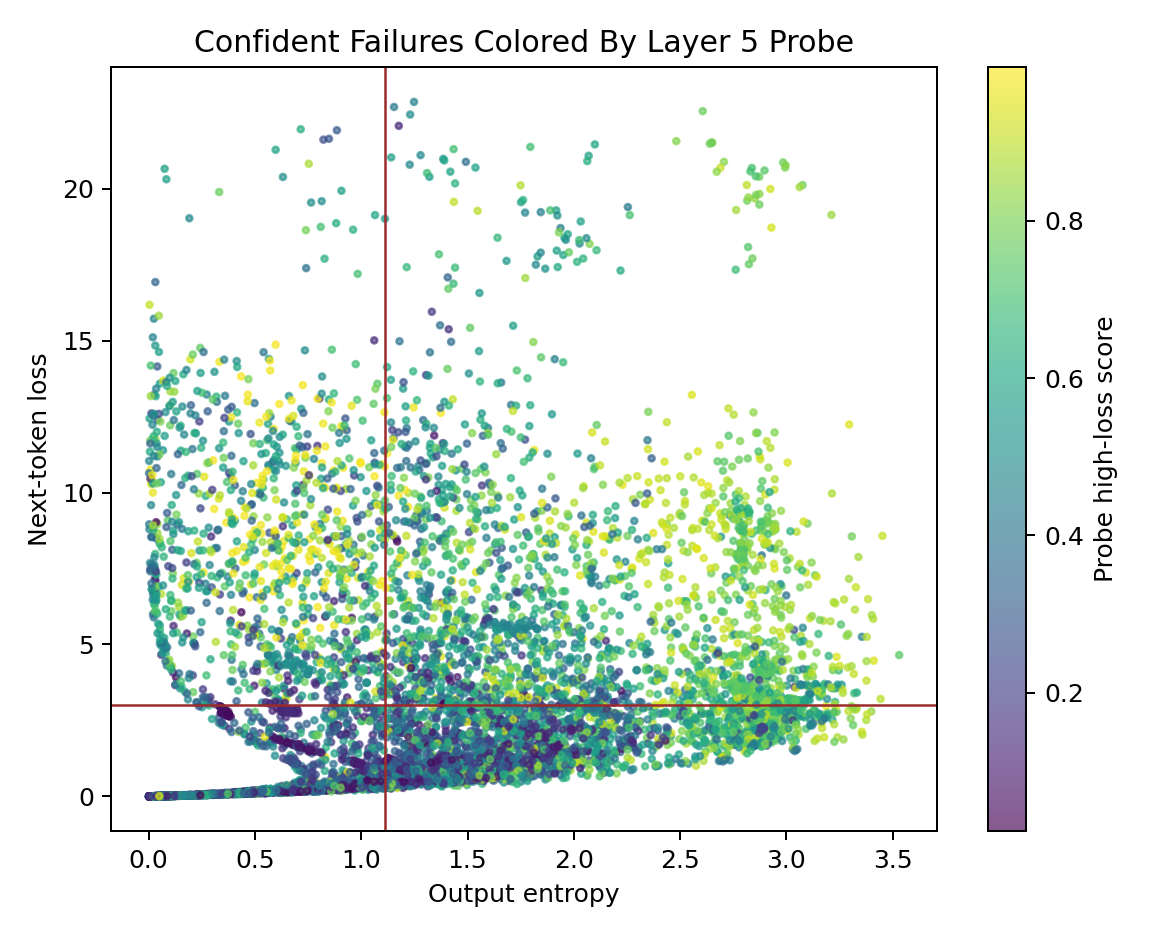
\includegraphics[width=0.78\linewidth]{../artifacts/plots/confident_failures_probe_score.png}
  \caption{Confident-failure tokens plotted by output entropy ($x$) and next-token loss ($y$), colored by layer-5 probe score. The upper-left region contains tokens where the model is confidently wrong: entropy is low, loss is high. Bright points in that region are cases where the residual-stream probe assigns a high trouble score despite low output entropy.}
  \label{fig:confident-failures}
\end{figure}

A representative caught example is from \texttt{ood\_char\_shuffle}: the target byte is \texttt{`t'}, the model's top prediction is \texttt{`E'}, the loss is $18.4$ nats, the entropy is $0.016$ nats (effectively zero), and the layer-5 probe score is $0.96$. The model's softmax is roughly maximally confident --- and wrong. The probe disagrees, correctly. We flag the obvious caveat: the probe used in this example was trained with \texttt{char\_shuffle} examples included, so this is an in-distribution catch under the seen-shift task, not a generalization claim. It illustrates the failure-mode geometry; the leave-one-shift-out tables above are the test of whether that geometry is recoverable from unseen shifts.

\section{Interpretation}

We can state what the data support without overstating it.

\paragraph{Within-distribution token surprise.}
On held-out Shakespeare alone, with no distribution shift to confound the result, the layer-4 logistic probe ranks high-loss tokens above ordinary tokens substantially better than output entropy ($0.779$ vs.\ $0.656$ AUROC). One framing of why this is possible at all: the map from the residual stream to the logits is deterministic, so any signal entropy has, the residual stream has by construction. Entropy is not a complete summary of the softmax --- it discards the mass-allocation information that distinguishes a sharp distribution on the wrong token (low entropy, high loss) from a sharp distribution on the right one. A linear probe on the residual stream can read features predictive of which positions tend to produce that pathology, and recover information that entropy aggregates away. Position effects, context difficulty, rare-token structure, and distributional weirdness are all plausible carriers of that signal. Informally, the model's internal state carries warning signs that its final confidence score does not expose. We resist the stronger claim that the model is in some intrinsic sense more uncertain than its softmax suggests --- a probe correlation does not establish that.

\paragraph{Seen-shift OOD versus generalization.}
The gap between the two OOD evaluations is the more telling result. Under the seen-shift task the probe is dominant ($0.879$ vs.\ $0.566$ AUROC); under leave-one-shift-out it beats entropy on $4$ of $5$ held-out families and loses on the cleanest one. This is the same failure mode that haunts probes built for deception, sycophancy, or jailbreak detection at the frontier: the probe overfits to the labeled failure families it was given, the in-distribution numbers look great, and the next failure type does not look like the previous ones along the directions the probe learned. Holding out a category at training time is what separates a curiosity from a deployable detector.

\paragraph{Detector choice depends on what you trust your training labels to cover.}
On the two LOSO settings where the supervised probe struggles most, the best detector is a one-class density estimator that has seen no OOD examples at all: Mahalanobis distance from the ID activation mean at layer~$0$--$1$. This is not a contradiction --- it is the expected behavior. A supervised probe is a directional detector; a Mahalanobis detector is radial in whitened activation space. When the held-out shift moves the activation along axes not represented in the labeled training shifts, the supervised probe loses ground but the radial detector still sees movement away from the ID cloud. The practical implication is that the right white-box monitor is shift-dependent, and that an OOD-free detector should be in the toolkit alongside trained probes rather than replaced by them.

\paragraph{Bayesian uncertainty.}
The diagonal-Laplace implementation does not add signal here. The result is conditional on two assumptions stacked together: the diagonal posterior and the fixed prior precision $\tau=1$. With $\tau=1$ and several thousand training rows, the posterior collapses tightly around the MAP solution; predictive-mean averaging then recovers the deterministic readout almost exactly regardless of whether the posterior is diagonal or full. A $\tau$ sweep would separate these two failure modes; we do not run it here.

\section{On the metaphor}

Imagine the model as a stagecoach driver crossing unfamiliar country. Its outputs are what it says out loud (``all clear ahead!''). Its activations are body language: tightened grip, eyebrow flicker. A probe is a passenger trained to read the body language and shout \emph{trouble} before the driver does. What we found in this small lab is that the body language really does leak information the words don't, and that a passenger trained on five kinds of bandits will sometimes miss the sixth, and that a passenger who only knows what a calm ride looks like sometimes spots the new bandit best. None of those sentences are about Shakespeare. They are the small forms of the questions a real white-box monitor for a frontier system has to answer.

\section{Related work and positioning}

DOWSING sits at the intersection of three established lines of work: linear probing of frozen representations (Alain and Bengio, 2016; Belinkov and Glass, 2019), representation-space OOD detection (Lee et al., 2018), and white-box monitoring as a precursor to mechanistic interpretability (Zou et al., 2023; Bricken et al., 2023; Cunningham et al., 2023). The contribution here is not methodological novelty. It is to reproduce the core monitoring loop --- training data, activations, labels, baselines, supervised probes, one-class detectors, and held-out shift evaluation --- in a model small enough that every step is inspectable from a laptop, and to report the negative results (Bayesian uncertainty under the diagonal-Laplace approximation; supervised probe failure on \texttt{char\_shuffle} under LOSO) at the same prominence as the positive ones. The intended use is as a teaching artifact and a calibration of expectations, not a benchmark.

\section{Scope}\label{sec:scope}

This is a project writeup at toy scale, not a formal benchmark paper. Three methodological items that a formal paper would address are out of scope for this artifact: validation-selected layer reporting, contiguous source-region splits, and bootstrap confidence intervals. We name them here rather than fold them into the general limitations list, so that a reader can see they were considered.

\paragraph{Test-split layer selection.} Layer-best tables in this paper report the layer that maximizes test-split AUROC for each detector (see \S\ref{sec:hyperparameters}). The validation split is held out from probe training but is not currently used for layer selection. A formal paper should select the layer on validation and report on test once. Doing so would likely lower some layer-best AUROCs relative to the descriptive sweeps reported here. The substantive question is whether the qualitative ordering --- supervised probe dominant in seen-shift OOD, Mahalanobis dominant on held-out \texttt{char\_shuffle} and \texttt{python} under LOSO, layer-4 logistic dominant on ID-only high-loss --- survives the change. We suspect it would often survive, because the LOSO setting already withholds substantial structure from probe training and recovers the same ordering, but we do not run the rerun here.

\paragraph{Window-level rather than source-region splits.} Splits are performed over fixed-length windows (\S\ref{sec:splits}). This prevents token-level leakage within a window, but neighboring windows from the same source byte stream can land in different splits when the stride is shorter than a full window. A stricter version of this experiment would partition the source corpus into contiguous regions before windowing, so that no two windows in different splits share any source bytes. This mainly affects the ID-only high-loss result, which should be read as a held-out-window result rather than a fully de-duplicated held-out-corpus result. The OOD evaluations are less affected because each shift family is generated from its own source stream.

\paragraph{No confidence intervals.} All AUROC values are point estimates. We report no bootstrap CIs over windows or sequences, so claims of the form ``probe beats entropy by $+0.123$ AUROC'' are not accompanied by an uncertainty bound. A formal version of this paper should include $95\%$ bootstrap confidence intervals (over evaluation windows or source sequences, $1{,}000$ resamples) for at least three headline rows: the ID-only high-loss probe vs.\ entropy, the seen-shift OOD probe vs.\ entropy, and the LOSO \texttt{char\_shuffle} row where the supervised probe loses to entropy and Mahalanobis recovers $0.696$ AUROC. Without those intervals, the relative magnitudes of the deltas reported in this paper are descriptive rather than tested.

\paragraph{What is and is not affected by these gaps.} All three fixes are mechanical: they change the rigor of the presentation, not the experimental design. The negative result for diagonal-Laplace uncertainty (predictive mean $\approx$ deterministic logistic; MI near or below chance) is unaffected, because that comparison is between two readouts of the same trained probe at the same layer, so layer selection, split policy, and resampling all cancel. The qualitative finding that supervised probes overfit to seen shift families --- and that an OOD-free Mahalanobis detector is the best deployable monitor on \texttt{char\_shuffle} and \texttt{python} under LOSO --- is similarly robust. The headlines that would benefit most are the within-distribution high-loss delta, where the gap between probe and entropy is narrower than the OOD gap, and any per-shift gain whose absolute size matters to a downstream claim.

\section{Limitations}

\begin{itemize}[topsep=2pt,itemsep=0pt]
  \item Tiny, undertrained byte-level model (validation loss $\sim 1.444$); single language-model seed and single split seed. The deltas reported in this paper are not equally robust to seed variation: the seen-shift OOD gap of $0.879$ vs.\ $0.566$ AUROC is large enough that a seed sweep is unlikely to reverse it, while the ID-only high-loss gap of $0.779$ vs.\ $0.656$ is small enough that a seed sweep would meaningfully sharpen or weaken how strongly the within-distribution claim should be read.
  \item Three of five OOD families (\texttt{python}, \texttt{modern\_prose}, \texttt{repetition}) are tiled templates that admit content memorization; the controlled \texttt{char\_shuffle} and \texttt{word\_shuffle} sets are the load-bearing OOD families.
  \item Aggregate OOD detection is a seen-shift task unless using the leave-one-type-out table.
  \item Original aggregate high-loss is partly confounded with OOD; the ID-only high-loss check is the cleaner token-surprise test.
  \item Diagonal Laplace posterior and fixed prior precision $\tau=1$ are stacked assumptions whose contributions a $\tau$ sweep should separate; see~\S\ref{sec:bayesian} for the diagnosis.
  \item Post-block residual hooks only; no embedding or final layer-norm probe.
  \item Position-in-window effects are not controlled.
  \item Probes are correlational, not causal.
\end{itemize}

\section{Future work}

Replace tiled synthetic OOD families with sampled corpora and de-duplicate windows across splits; promote leave-one-shift-out to the primary OOD metric; add bootstrap confidence intervals and repeat across LM and split seeds; evaluate high-loss within ID and within each OOD family separately; add embedding and final-layer-norm probes; test causal interventions along learned probe directions; compare against sparse autoencoder features; extend to generation-time monitoring of full samples rather than per-token labels.

\section{Conclusion}

The headline finding of this small lab is that the right white-box detector depends on what its training labels are expected to cover. A supervised linear probe on residual-stream activations dominates in the seen-shift OOD regime ($0.879$ vs.\ $0.566$ AUROC) and continues to beat output entropy on $4$ of $5$ held-out shift families under leave-one-shift-out, but loses on character-shuffled Shakespeare when that family is withheld from training. On exactly the held-out shifts where the trained probe struggles --- \texttt{char\_shuffle} and \texttt{python} --- an OOD-free Mahalanobis density estimator on early-layer activations becomes the best deployable detector. The gap between these two regimes, more than either result on its own, is what the experiment teaches: directional supervised detectors and radial unsupervised detectors do different jobs, and the choice between them must be matched to the failure families a deployer expects to encounter.

A separate, cleaner positive result on within-distribution surprise: with no shift to confound the comparison, a layer-4 logistic probe reaches $0.779$ AUROC on ID-only high-loss tokens versus $0.656$ for entropy. This says, mechanically, that entropy discards mass-allocation information present in the residual stream, and that a linear probe can recover some of what entropy aggregates away.

The diagonal-Laplace Bayesian probe did not add signal in this implementation, conditional on two stacked assumptions --- diagonal posterior and fixed prior precision $\tau=1$ --- whose contributions a future $\tau$ sweep should separate. The dowsing rod twitches; we are interested in when, and over what.

\paragraph{Reproducibility.}
{\sloppy
Run metadata: Modal NVIDIA L4 GPU; $3{,}000$ training iterations; batch size $64$; block size $128$; $6$ layers, $6$ heads, $192$ embedding dim; byte vocabulary; $\sim 50{,}000$ target tokens per eval set. Artifact bundle: \path{modal_outputs/full-l4-3000-robustness-dowsing-results.tar.gz}. Source code: see \texttt{src/}, \texttt{scripts/}, and \texttt{lab/} in the repository.\par}

\section*{References}

\begin{itemize}[leftmargin=*,topsep=2pt,itemsep=2pt]
  \item Alain, G.\ and Bengio, Y.\ (2016). \emph{Understanding intermediate layers using linear classifier probes.} arXiv:1610.01644.
  \item Belinkov, Y.\ and Glass, J.\ (2019). \emph{Analysis methods in neural language processing: A survey.} TACL.
  \item Lee, K., Lee, K., Lee, H., and Shin, J.\ (2018). \emph{A Simple Unified Framework for Detecting Out-of-Distribution Samples and Adversarial Attacks.} NeurIPS.
  \item MacKay, D.\ J.\ C.\ (1992). \emph{A practical Bayesian framework for backpropagation networks.} Neural Computation.
  \item Karpathy, A.\ (2022). \emph{nanoGPT.} \texttt{github.com/karpathy/nanoGPT}.
  \item Bricken, T.\ et al.\ (2023). \emph{Towards Monosemanticity.} Anthropic.
  \item Cunningham, H.\ et al.\ (2023). \emph{Sparse Autoencoders Find Highly Interpretable Features in Language Models.} arXiv:2309.08600.
  \item Zou, A.\ et al.\ (2023). \emph{Representation Engineering: A Top-Down Approach to AI Transparency.} arXiv:2310.01405.
\end{itemize}

\clearpage
\appendix

\section{Per-shift seen-shift breakdown (numbers behind Figure~\ref{fig:typebreakdown})}\label{app:typebreakdown}

Numbers behind Figure~\ref{fig:typebreakdown} in the main text. The probe beats entropy on every family; the leave-one-shift-out evaluation (Table~\ref{tab:loso} in the main text) shows that some of these gains do not survive when the family is withheld from training.

\begin{center}
  \small
  \begin{tabular}{lccc}
    \toprule
    OOD family & Layer-5 probe AUROC & Entropy AUROC & $\Delta$ \\
    \midrule
    \texttt{repetition}    & 0.962 & 0.505 & $+0.457$ \\
    \texttt{modern\_prose} & 0.901 & 0.571 & $+0.330$ \\
    \texttt{python}        & 0.920 & 0.591 & $+0.329$ \\
    \texttt{word\_shuffle} & 0.832 & 0.554 & $+0.279$ \\
    \texttt{char\_shuffle} & 0.774 & 0.603 & $+0.171$ \\
    \bottomrule
  \end{tabular}
\end{center}

\end{document}
